\newpage
\section{Appendix A: MatLab Code}

\subsection{Part 1 - Identification of boat parameters}
\begin{lstlisting}
%% 1b Simulating in calm water(no disturbances) and identification of parameter T and K
omega = 0.005; %rad/s w_1
A=1;           %Amplitude
simTime = 1000; % [s]
simout = sim('ship1b','startTime','0','stopTime',sprintf('%d',simTime));
time = simout.get('time');     %get time from workspace
psi_w1 = simout.get('psi'); %get psi from workspace

% run the simulation with  w_2
omega = 0.05; %[rad/s] w_2
A=1;          %Amplitude

simTime = 1000; % [s]
simout = sim('ship1b','startTime','0','stopTime',sprintf('%d',simTime));
time = simout.get('time');     %get time from workspace
psi_w2 = simout.get('psi'); %get psi from workspace

%plotting into one window
subplot(2,1,1)
plot(time,psi_w1)
xlabel('t [s]')
ylabel('$\psi$ [deg]')
title('Simulation with $\omega_1=0.005$   (No Noise on measurement)')
legend('\psi (average heading) ', 'Location','SouthEast')
grid on;
subplot(2,1,2)
plot(time,psi_w2)
xlabel('t [s]')
ylabel('$\psi$ [deg]')
title('Simulation with $\omega_w=0.05$   (No Noise on measurement)')
legend('\psi (average heading) ', 'Location','SouthEast')
grid on;

%%code that identifies the T and K value


%% 1c: Simulating in rough weather(Waves+Noise) Amplitude=1
omega = 0.005; %rad/s %w_1
A=1;           %Amplitude
simTime = 1000; % [s]
simout = sim('ship1c','startTime','0','stopTime',sprintf('%d',simTime));
time = simout.get('time');     %get time from workspace
psi_w1_rough = simout.get('psi'); %get psi from workspace

%simulate again for w_2
omega = 0.05;  %rad/s %w_w
A=1;           %Amplitude
simTime = 1000; % [s]
simout = sim('ship1c','startTime','0','stopTime',sprintf('%d',simTime));
time = simout.get('time');     %get time from workspace
psi_w2_rough = simout.get('psi'); %get psi from workspace

%Ploting the figures
subplot(2,1,1)
plot(time,psi_w1_rough)
xlabel('t [s]')
ylabel('$\psi$ [deg]')
title('Simulation with $\omega_1=0.005$  (With waves and measurement noise) ')
legend('\psi + \psi_{w} (average heading +  wave disturbances) ', 'Location','SouthEast')
grid on;
subplot(2,1,2)
plot(time,psi_w2_rough)
xlabel('t [s]')
ylabel('$\psi$ [deg]')
title('Simulation with $\omega_w=0.05$   (With waves and measurement noise)')
legend('\psi + \psi_{w} (average heading +  wave disturbances) ', 'Location','SouthEast')
grid on;


%% 1c: simulation in rough weather (waves+noise) with higher amplitude A=45

omega = 0.005; %rad/s %w_1
A=45;           %Amplitude
simTime = 1000; % [s]
simout = sim('ship1c','startTime','0','stopTime',sprintf('%d',simTime));
time = simout.get('time');     %get time from workspace
psi_w1_rough_A45 = simout.get('psi'); %get psi from workspace

%simulate again for w_2
omega = 0.05;  %rad/s %w_w
A=45;           %Amplitude
simTime = 1000; % [s]
simout = sim('ship1c','startTime','0','stopTime',sprintf('%d',simTime));
time = simout.get('time');     %get time from workspace
psi_w2_rough_A45 = simout.get('psi'); %get psi from workspace

%Plotting the figures
subplot(2,1,1)
plot(time,psi_w1_rough_A45)
xlabel('t [s]')
ylabel('$\psi$ [deg]')
title('Simulation with $\omega_1=0.005$ and $A=45$   (With waves and measurment noise) ')
legend('\psi + \psi_{w} (average heading +  wave disturbances) ', 'Location','SouthEast')
grid on;
subplot(2,1,2)
plot(time,psi_w2_rough_A45)
xlabel('t [s]')
ylabel('$\psi$ [deg]')
title('Simulation with $\omega_w=0.05$ and $A=45$   (With waves and measurment noise)')
legend('\psi + \psi_{w} (average heading +  wave disturbances) ', 'Location','SouthEast')
grid on;

%% 1d: Comparison of all models
%Make The Transfer Functions 
num1=[0.1742];       %with K
den1=[86.52685 1 0]; %with T
H1=tf(num1,den1);    %No noise Transfer Function

num2=[0.1734];       %with K
den2=[84.3920 1 0];  %with T
H2=tf(num2,den2);    %With noise Transfer Function

%simulate
simTime = 1000; % [s]
simout = sim('ship1d','startTime','0','stopTime',sprintf('%d',simTime));
time = simout.get('time');
psi_s = simout.get('psi'); %system
psi_no_noise = simout.get('psi_no_noise'); %model with no noise
psi_with_noise = simout.get('psi_with_noise'); %model with noise

%draw plot
plot(time,psi_s,'r',time,psi_with_noise,'b',time,psi_no_noise,'g')
xlabel('t [s]')
ylabel('$\psi$ [deg]')
legend('Ship','Model (calm)','Model (rough)','Location','southeast')
title('Step response of models and system')
grid on
\end{lstlisting}

\subsection{Part 2 - Identification of wave spectrum model}
\begin{lstlisting}
%% 2a: Estimate PSD
load('wave.mat');       % Load wave disturbance

F_s = 10;
window = 4096;
noverlap = [];
nfft = [];
[S_psi,f] = pwelch(psi_w(2,:).*(pi/180),window,noverlap,nfft,F_s);
omega = 2*pi.*f;
S_psi = S_psi./(2*pi);


%% 2c: Find omega_0
% Plot estimated PSD

plot(omega,S_psi, 'LineWidth', 2)
axis([0 2 -0.00005 16*10^(-4)])
hold on
xlabel('$\omega$ [$\frac{rad}{s}$]')
ylabel('$S_{\psi_{w}}(\omega)$ [rad]')
title(['Estimated power spectral density fuction of $S_{\psi_{w}}(\omega)$ '...
    ])
grid on;


%% 2c: Find resonance frequency from estimated PSD)
[maxPSD,  frequency_index ] = max( S_psi )
omega_0 = omega( frequency_index )

%% 2d: Comparison
sigma = sqrt(maxPSD); % sigma_squared is the peak value of S_psi_w

%using lsqcurvefit

P_psi = @(lambda,omega) ...
    (4*lambda^2*omega_0^2*sigma^2*omega.^2) ./ ...
    (omega.^4 + (2*lambda^2 - 1)*2*omega_0^2*omega.^2 + ...
    omega_0^4);

lambda0 = 10;
lb=0;
ub=10;

lambda = lsqcurvefit(P_psi,lambda0,omega,S_psi,lb,ub);
P_psi = P_psi(lambda,omega);
K_w = 2*lambda*omega_0*maxPSD;

%%% Comparison plot of estimate and analytical
figure
plot(omega, P_psi, 'r')
hold on
plot(omega, S_psi, 'b')
legend('P_{\psi_w}','S_{\psi_w}')
xlim([0 2])
xlabel('t [s]')
ylabel('PSD [deg^2/(rad/s)')
title('Comparison of estimated PSD function $(S_{\psi_w})$ and the analytical $P_{\psi_w}$');
grid on;

\end{lstlisting}

\subsection{Part 3 - Control system design}
\begin{lstlisting}
%%From earlier excercies 
K=0.1734;
T=84.3920;
%% 5.3a
w_c=0.1; %cutoff frequency [rad/s]
PM=50/180*pi;%Phase margin [rad]
T_d=T;        %chosen such that it cancels the TF time constant
%Make transfer function for controller
T_f=1/(tan(PM)*w_c);    
K_pd=sqrt((T_f^2*w_c^4+w_c^2)/K^2);
num_controller=[K_pd*T_d,K_pd];
den_controller=[T_f,1];

H_pd=tf(num_controller,den_controller); %make transfer function for controller

%%Make transfer function for plant
H_ship=tf([K],[T 1 0]);                 %transfer function for plant

%open-loop system
H_ol=H_pd*H_ship;                       %Open loop transfer function

%draw a bode idagram
figure
bode(H_ol);
grid ;
title('Bode plot for the open-loop system H_ol(s)');



%% 5.3b)

ref=30;
simTime=400; 

simout = sim('ship3b','startTime','0','stopTime',sprintf('%d',simTime));
time = simout.get('time');     %get time from workspace
psi = simout.get('psi'); %get psi from workspace
ref=simout.get('ref');
%error=simout.get('error'); % no need for this, not gonna plot it.
delta=simout.get('rudder_input');

%Ploting the graphs
figure
plot(time,ref,'black--',time,psi,time,delta) %plots time against refrence, output and rudder_input
legend('\psi_r(t)','\psi(t)','\delta(t)','location','Southeast')
xlabel('t[s]');
ylabel('\psi_r(t), \psi(t), \delta(t) [deg]'); 
title('Autopilot without current or wave disturbances')
%make y-axis formating become less
grid on;

%% 5.3c)

ref=30;
simTime=400; 

simout = sim('ship3c','startTime','0','stopTime',sprintf('%d',simTime));
time = simout.get('time');     %get time from workspace
psi = simout.get('psi'); %get psi from workspace
ref=simout.get('ref');
%error=simout.get('error'); % no need for this, not gonna plot it.
delta=simout.get('rudder_input');

%Ploting the graphs
figure
plot(time,ref,'black--',time,psi,time,delta) %plots time against refrence, output and rudder_input
legend('\psi_r(t)','\psi(t)','\delta(t)','location','Southeast')
xlabel('t[s]');
ylabel('\psi_r(t), \psi(t), \delta(t) [deg]'); 
title('Autopilot with current disturbances')
%make y-axis formating become less
grid on;

%% 5.3d)

ref=30;
simTime=400; 

simout = sim('ship3d','startTime','0','stopTime',sprintf('%d',simTime));
time = simout.get('time');     %get time from workspace
psi = simout.get('psi'); %get psi from workspace
ref=simout.get('ref');
%error=simout.get('error'); % no need for this, not gonna plot it.
delta=simout.get('rudder_input');

%Ploting the graphs
figure
plot(time,ref,'black--',time,psi,time,delta) %plots time against refrence, output and rudder_input
legend('\psi_r(t)','\psi(t)','\delta(t)','location','Southeast')
xlabel('t[s]');
ylabel('\psi_r(t), \psi(t), \delta(t) [deg]'); 
title('Autopilot with wave disturbances')
%make y-axis formating become less
grid on;


\end{lstlisting}

\subsection{Part 4- Observability}
\begin{lstlisting}
load('constants');
%% 5.4a): Finding the matrices
A = [0 1 0 0 0; -omega_0^2 -2*lambda*omega_0 0 0 0; 0 0 0 1 0; ...
    0 0 0 -1/T -K/T; 0 0 0 0 0];
B = [0; 0; 0; K/T; 0];
C = [0 1 1 0 0];
E = [0 0; K_w 0; 0 0; 0 0; 0 1];

%% 5.4b): Observabillity without disturbances
A = [0 1; 0 -1/T];
B=[0; K/T];
C= [1 0];
O = obsv(A,C);
rank(O) % rank(O) = 2 == n -> observable

%% 5.4c) Observabillity with current
A_b = [0 1 0; 0 -1/T -K/T; 0 0 0]; 
C_b = [1 0 0];
O_b = obsv(A_b,C_b);
rank(O_b)   %rank(O_b) = 3 == n -> observable


%% 5.4d) Observabillity with waves 
A_w = [0 1 0 0; -omega_0^2 -2*lambda*omega_0 0 0; 0 0 0 1; 0 0 0 -1/T];
C_w = [0 1 1 0];
O_w = obsv(A_w,C_w);
rank(O_w) % rank(Ob) = 4 == n -> observable

%% 5.4e) Observabillity with current and wave
O_cw = obsv(A,C); % rank(Ob) = 5 == n -> observable

\end{lstlisting}

%%%%%%%%%%%%%%%%%%%%%%%%%%%%%%%%%%%%%%%%%%%%%%%%%%%%%%%%%%%%%%%%%%%%%%%%%%%%%%%%%%%%%%%%%%%%%
% PART 5 - DISCRETE KALMAN FILTER
%%%%%%%%%%%%%%%%%%%%%%%%%%%%%%%%%%%%%%%%%%%%%%%%%%%%%%%%%%%%%%%%%%%%%%%%%%%%%%%%%%%%%%%%%%%%%

\subsection{Part 5 - Discrete Kalman filter function}

\begin{lstlisting}
function [b,psi] = fcn(u, y, data)

persistent init_flag A B C E Q R P_ x_ I 

if (isempty(init_flag))
    init_flag = 1;
    
    % Initialization for system
    [A,B,C,E,Q,R,P_,x_, I] = deal(data.Ad,data.Bd,data.Cd,data.Ed,data.Q, ...
                                data.R, data.P_0, data.X_0, data.I);
end

% 1 - Compute the Kalman Gain
    L = (P_*C')/((C*P_*C'+R));
% 2 - Update estimate with measurment
    x = x_ + L*(y-C*x_);
% 3 - Update error covariance matrix
    P = (I - L*C)*P_*(I-L*C)'+L*R*L';
% 4 - go to next
    x_ = A*x + B*u;
    P_ = A*P*A' + E*Q*E';

psi = x(3); b = x(5);
\end{lstlisting}

\begin{lstlisting}
%% 5.1a): 
load('constants');

%Make transfer function for controller
T_f=1/(tan(PM)*w_c);    
K_pd=sqrt((T_f^2*w_c^4+w_c^2)/K^2);
num_controller=[K_pd*T_d,K_pd];
den_controller=[T_f,1];

% Discretize model
A = [0 1 0 0 0; -omega_0^2 -2*lambda*omega_0 0 0 0; 0 0 0 1 0; ...  
    0 0 0 -1/T -K/T; 0 0 0 0 0];
B = [0; 0; 0; K/T; 0];
C = [0 1 1 0 0];
D = 0;
E = [0 0; K_w 0; 0 0; 0 0; 0 1];

f_s=10;         % Sampling frequency [Hz]
T_s = 1/f_s;    % Sampling time [s]

% Discretize model 
[Ad,Bd] = c2d(A,B,T_s);
% Discretize model 
[~,Ed] = c2d(A,E,T_s);
Cd=C;

%% 5b: measure variance 

simTime = 600; % [s]
simout = sim('ship5b','startTime','0','stopTime',sprintf('%d',simTime)); % no noise
psi = simout.get('compass'); 
R = var(psi*pi/180);    

%% 5c: Discrete Kalman Filter

Q = [30 0; 0 10^(-6)];
R = R/T_s;
P_0 = [1 0 0 0 0; 0 0.013 0 0 0; 0 0 pi^2 0 0; 0 0 0 1 0;  0 0 0 0 2.5*10^-4];
X_0 = [0; 0; 0; 0; 0];
I = diag([1 1 1 1 1]);

% data struct to use in matlab function
 data = struct('Ad',Ad,'Bd',Bd,'Cd',Cd,'Ed', Ed, 'Q',Q,'R', R,'P_0',P_0,'X_0',X_0, 'I', I);
 
 
 %% 5d: Feed forward estimated bias
 
load_system('ship5d.slx')
sim('ship5d.slx')

% Plot measured compass with and without estimated bias
figure(figNum)
figNum = figNum+1;
subplot(2,1,1)
plot(time,ref, 'r--', time, compass, time, compass_kalman)
title(['Reference $\psi_{r} = 30$, measured $\psi$ with and'...
' without Kalman-estimated bias $\hat{b}$']);
xlabel('t [s]'); 
ylabel('Angle [deg]');
legend({'$\psi_{r}$', '$\psi$ with $\hat{b}_{feedforward}$', ...
    '$\psi$ without $\hat{b}_{feedforward}$'},   ...
    'Interpreter', 'latex', 'Location', 'best')
grid  on ;

subplot(2,1,2)
plot(time, bias,'m', time, rudder_input, time, rudder_input_2)
title(['Kalman-estimated bias $\hat{b}$, and rudder input $\delta$ ' ...
'with and without Kalman-estimated bias $\hat{b}$'], ...
 'Interpreter', 'latex');
xlabel('t [s]');
ylabel('Angle [deg]');
legend({'$\hat{b}$', '$\delta$ with $\hat{b}_{feedforward}$', ...
    '$\delta$ without $\hat{b}_{feedforward}$'},   ...
    'Interpreter', 'latex', 'Location', 'best')
grid on;


%% 5e: Feed forward estimated bias and wave filtered psi
load_system('ship5e.slx')
sim('ship5e.slx')


load_system('ship5e.slx')
sim('task5_5_e.slx')

%Plot measured compass and estimated compass
figure(figNum)
figNum = figNum+1;
plot(t,sim_PSI_r, 'r--', t, sim_compass, t, psi_filtered)
title(['Reference $\psi_{r} = 30, measured $\psi$ $\psi + \psi_{w} + v and estimated course \hat{\psi}']);
xlabel('t [s]');
ylabel('Angle [deg]');
legend({'\psi_{r}', 'measured compass course ($\psi$ + $\psi_{w} $+ $v$)' , 'estimated compass course ($\hat{\psi}$)'}, 'Location', 'best')
 grid on; 

 
%Plot measured psi with and without Kalman filtered bias and waves
figure(figNum)
figNum = figNum+1;
plot(t,sim_PSI_r, 'r--', t, sim_compass,'b', t3, psi3,'g')
title('Compass reference \psi_{r} = 30, and measured compass course', ...
   'Interpreter', 'latex');
xlabel('t [s]'); 
ylabel('Angle [deg]');
legend({'$\psi_{r}$', 'With Kalman filtered feedback', ...
    'Without Kalman filtered feedback'},  ...
    'Interpreter', 'latex', 'Location', 'best')
grid on; 

%Plotting delta (rudder input)
figure(figNum)
figNum = figNum+1;
subplot(2,1,1)
plot(time, bias,'m', time,rudder_input)
title('Rudder input $\delta$ and estimated bias $\hat{b}$', ...
     'Interpreter', 'latex');
xlabel('t [s]');
ylabel('Angle [deg]');
legend({'$\hat{b}$', '\delta'},  ...
    'Interpreter', 'latex', 'Location', 'best')
grid on;

subplot(2,1,2)
plot(time, rudder_input)
title(['Rudder input $\delta$ without Kalman filtered $\hat{\psi}$ '...
    'or $\hat{b}$'], 'Interpreter', 'latex');
xlabel('t [s]'); 
ylabel('Angle [deg]');
legend({'$\delta$'}, 'Interpreter', 'latex', 'Location', 'best')
grid on;


% Wave influence (current turned off, delta = 0)
load_system('ship5e_1.slx')  
sim('ship5e_1.slx')

% Plotting wave influence on system
figure(figNum)
figNum = figNum+1;
plot(time, compass, time, compass_kalman)
title(['Measured wave influence \psi_{w} vs. estimated wave influence'...
    ' \hat{\psi}_{w}'],'Interpreter', 'latex');
xlabel('t [s]'); 
ylabel('Angle [deg]');
legend({'$\psi_{w}$', '$\hat{\psi}_{w}$'},  ...
    'Interpreter', 'latex', 'Location', 'best')
grid on;
 
\end{lstlisting}

%%%%%%%%%%%%%%%%%%%%%%%%%%%%%%%%%%%%%%%%%%%%%
% CONTINUE WITH ALL THE MATLAB CODE BEFORE SECTION: SimuLink Models
%%%%%%%%%%%%%%%%%%%%%%%%%%%%%%%%%%%%%%%%%%%%%
\newpage
\section{Appendix B: Simulink Models}

\begin{figure}[!htb]
    \caption{Simulink model from section 1.2/1.3}
    \centering
    \centerline{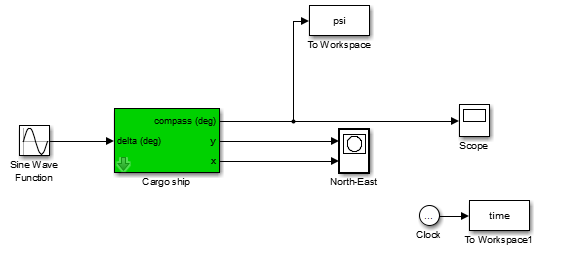
\includegraphics[scale=0.6]{simulink/sim1bc}}
    \label{simulink:1b}
\end{figure}

\begin{figure}[!htb]
    \caption{Simulink model from section 3.3/3.4}
    \centering
    \centerline{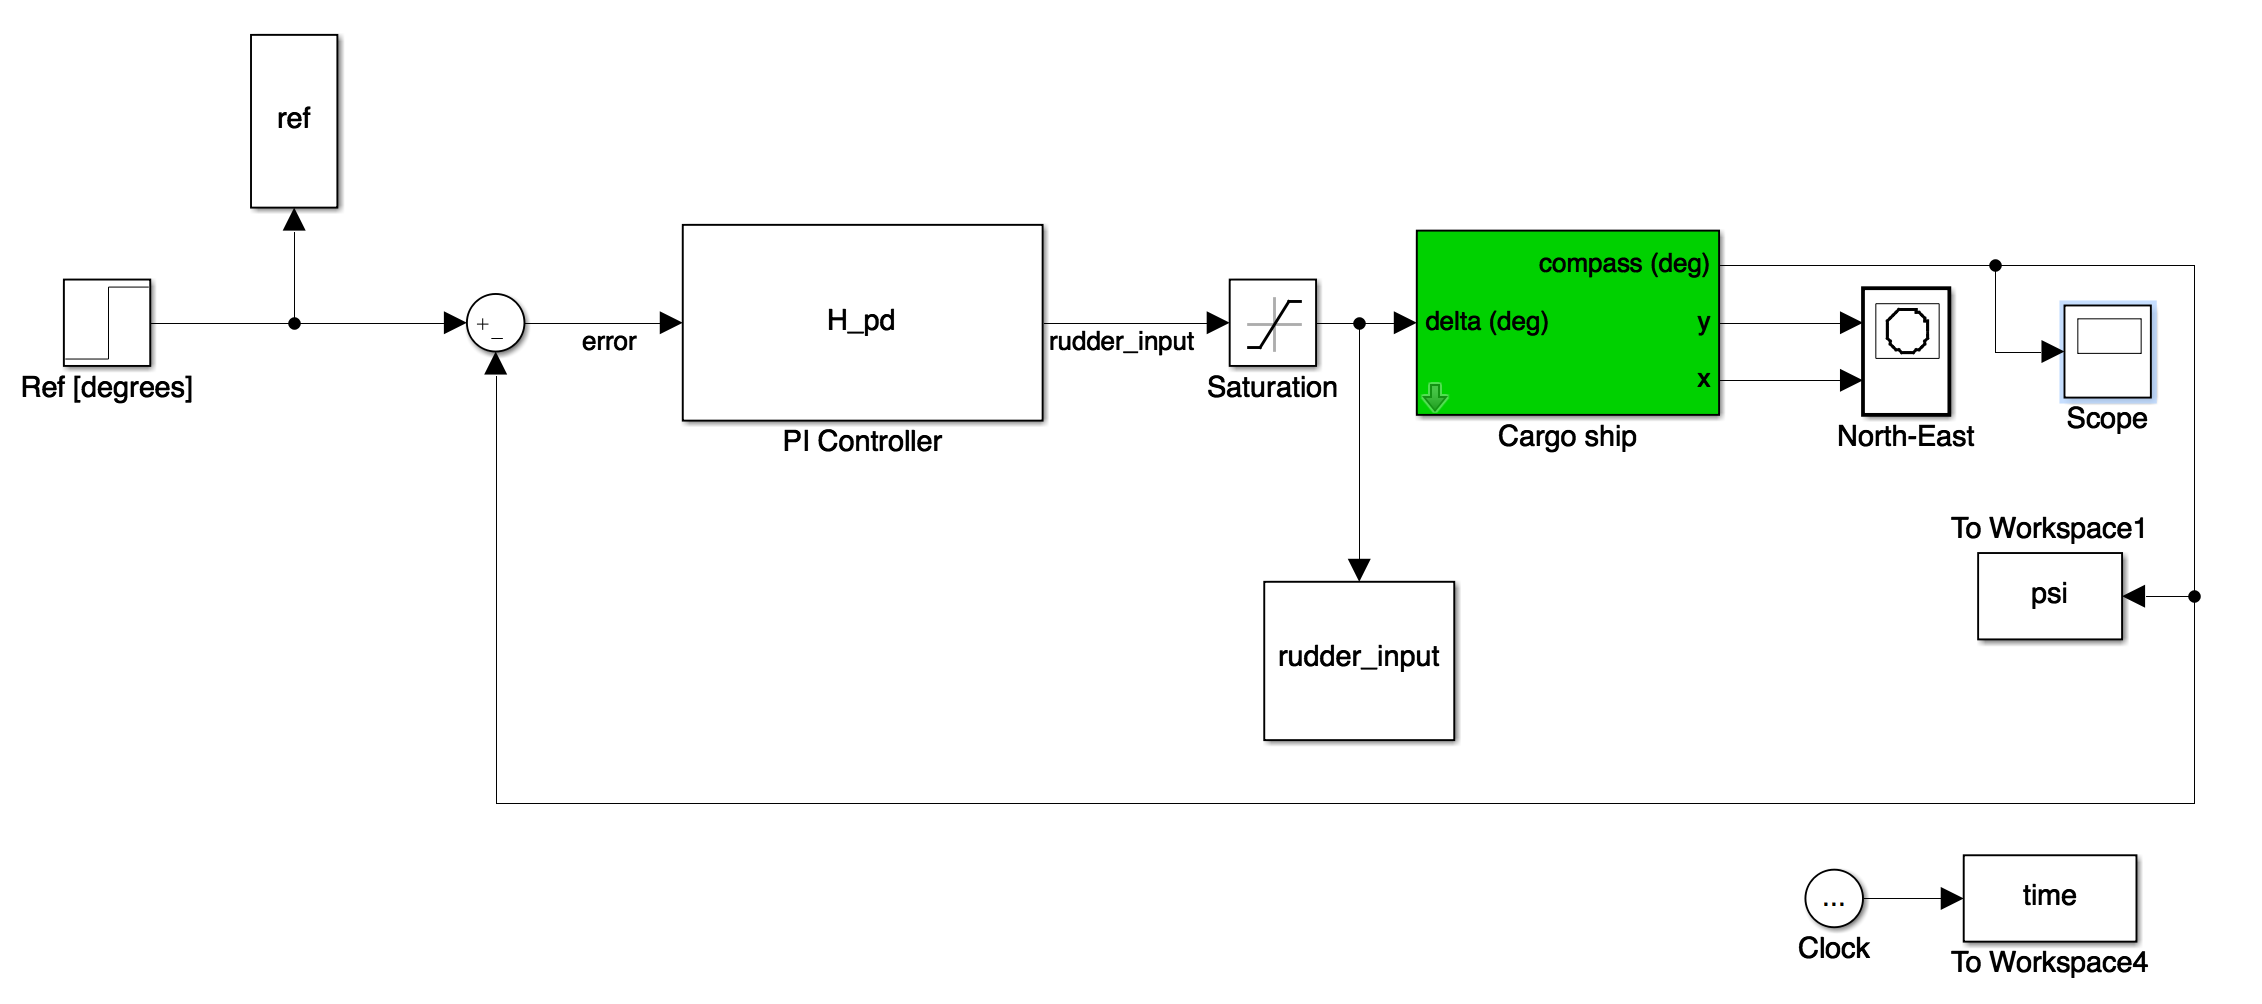
\includegraphics[scale=0.3]{simulink/sim3cd}}

\end{figure}

\begin{figure}[!htb]
    \caption{Simulink model from section 5.2}
    \centering
    \centerline{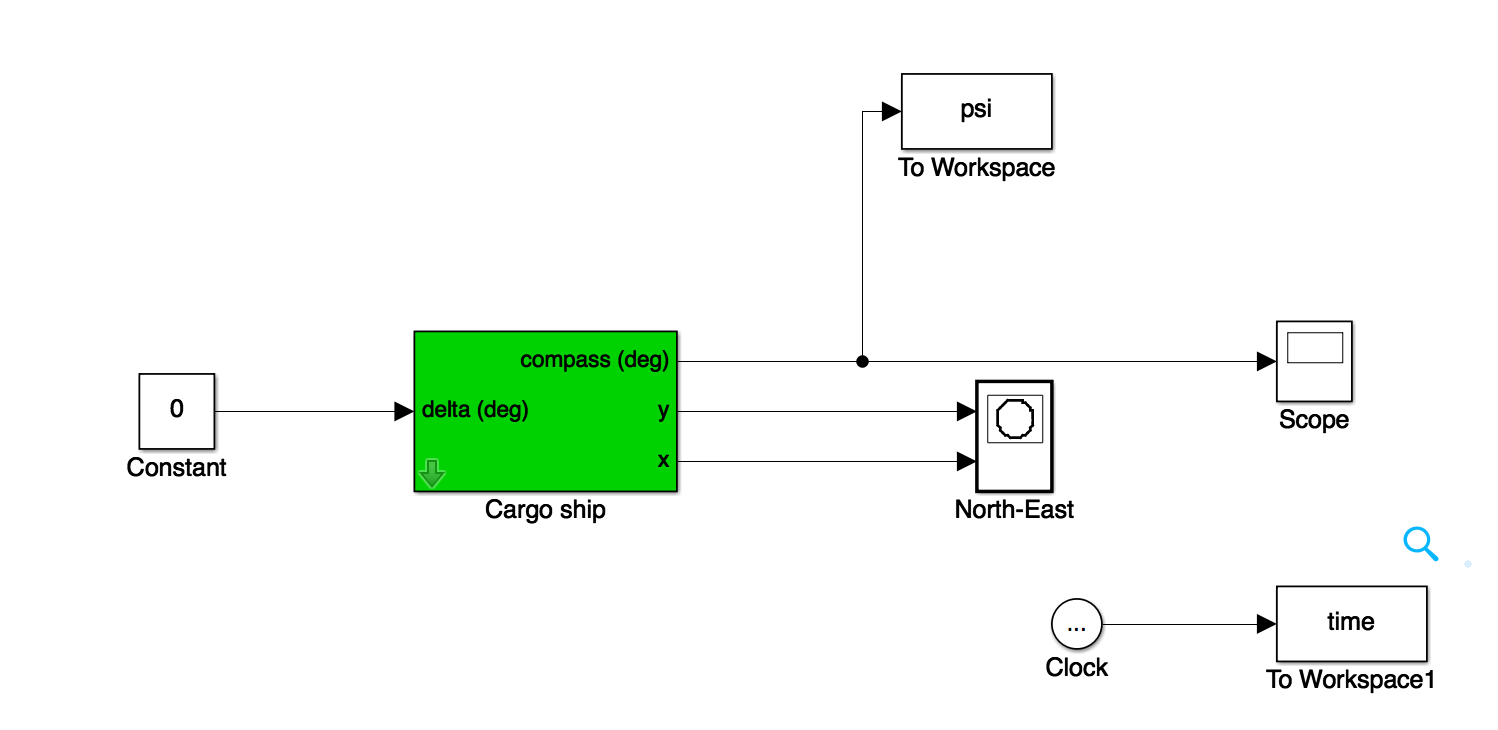
\includegraphics[scale=0.3]{simulink/sim5b}}

\end{figure}

\begin{figure}[!htb]
    \caption{Simulink model from section 5.4}
    \centering
    \centerline{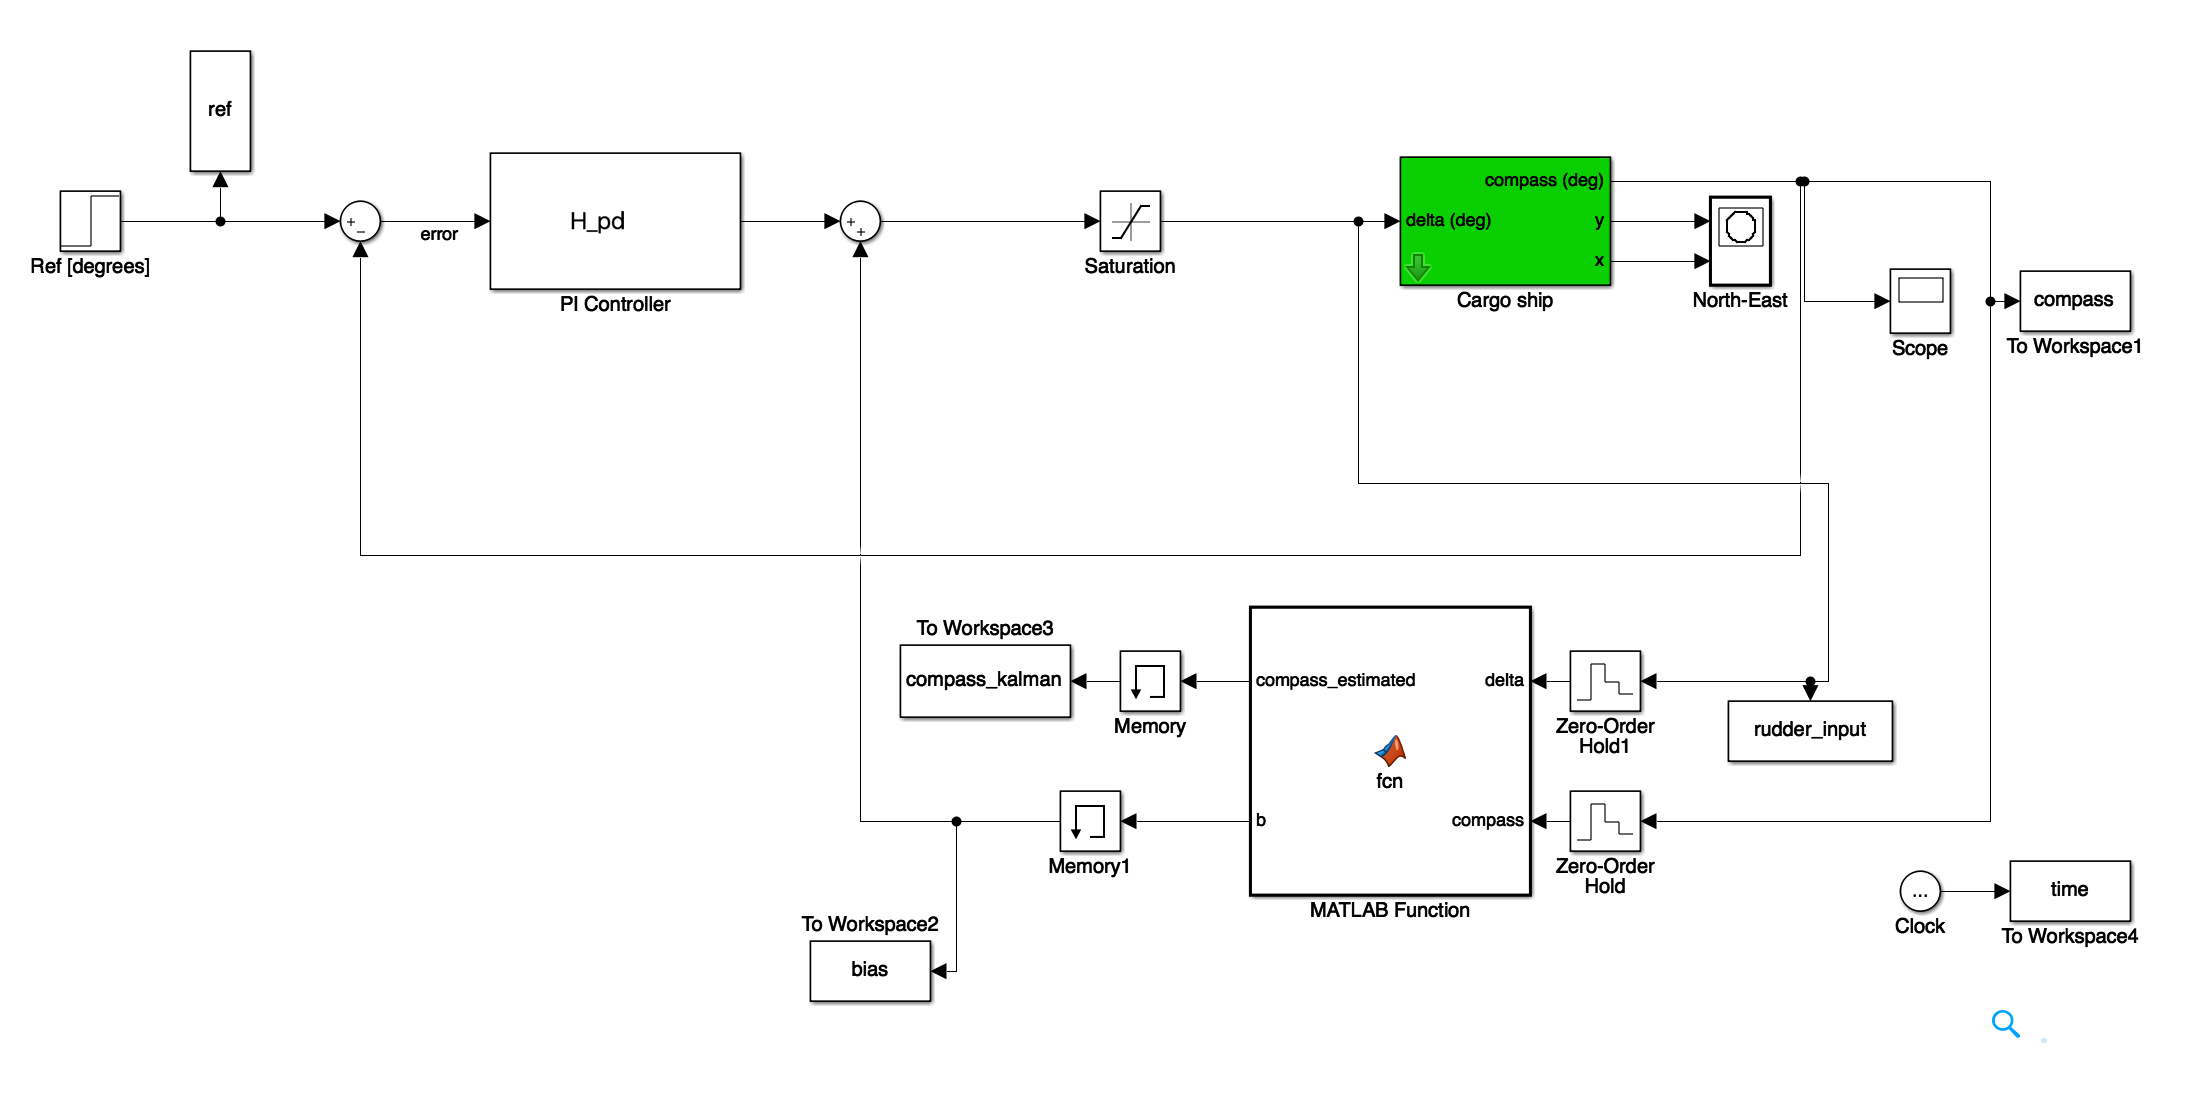
\includegraphics[scale=0.3]{simulink/sim5d}}

\end{figure}

\begin{figure}[!htb]
    \caption{Simulink model from section 5.5}
    \centering
    \centerline{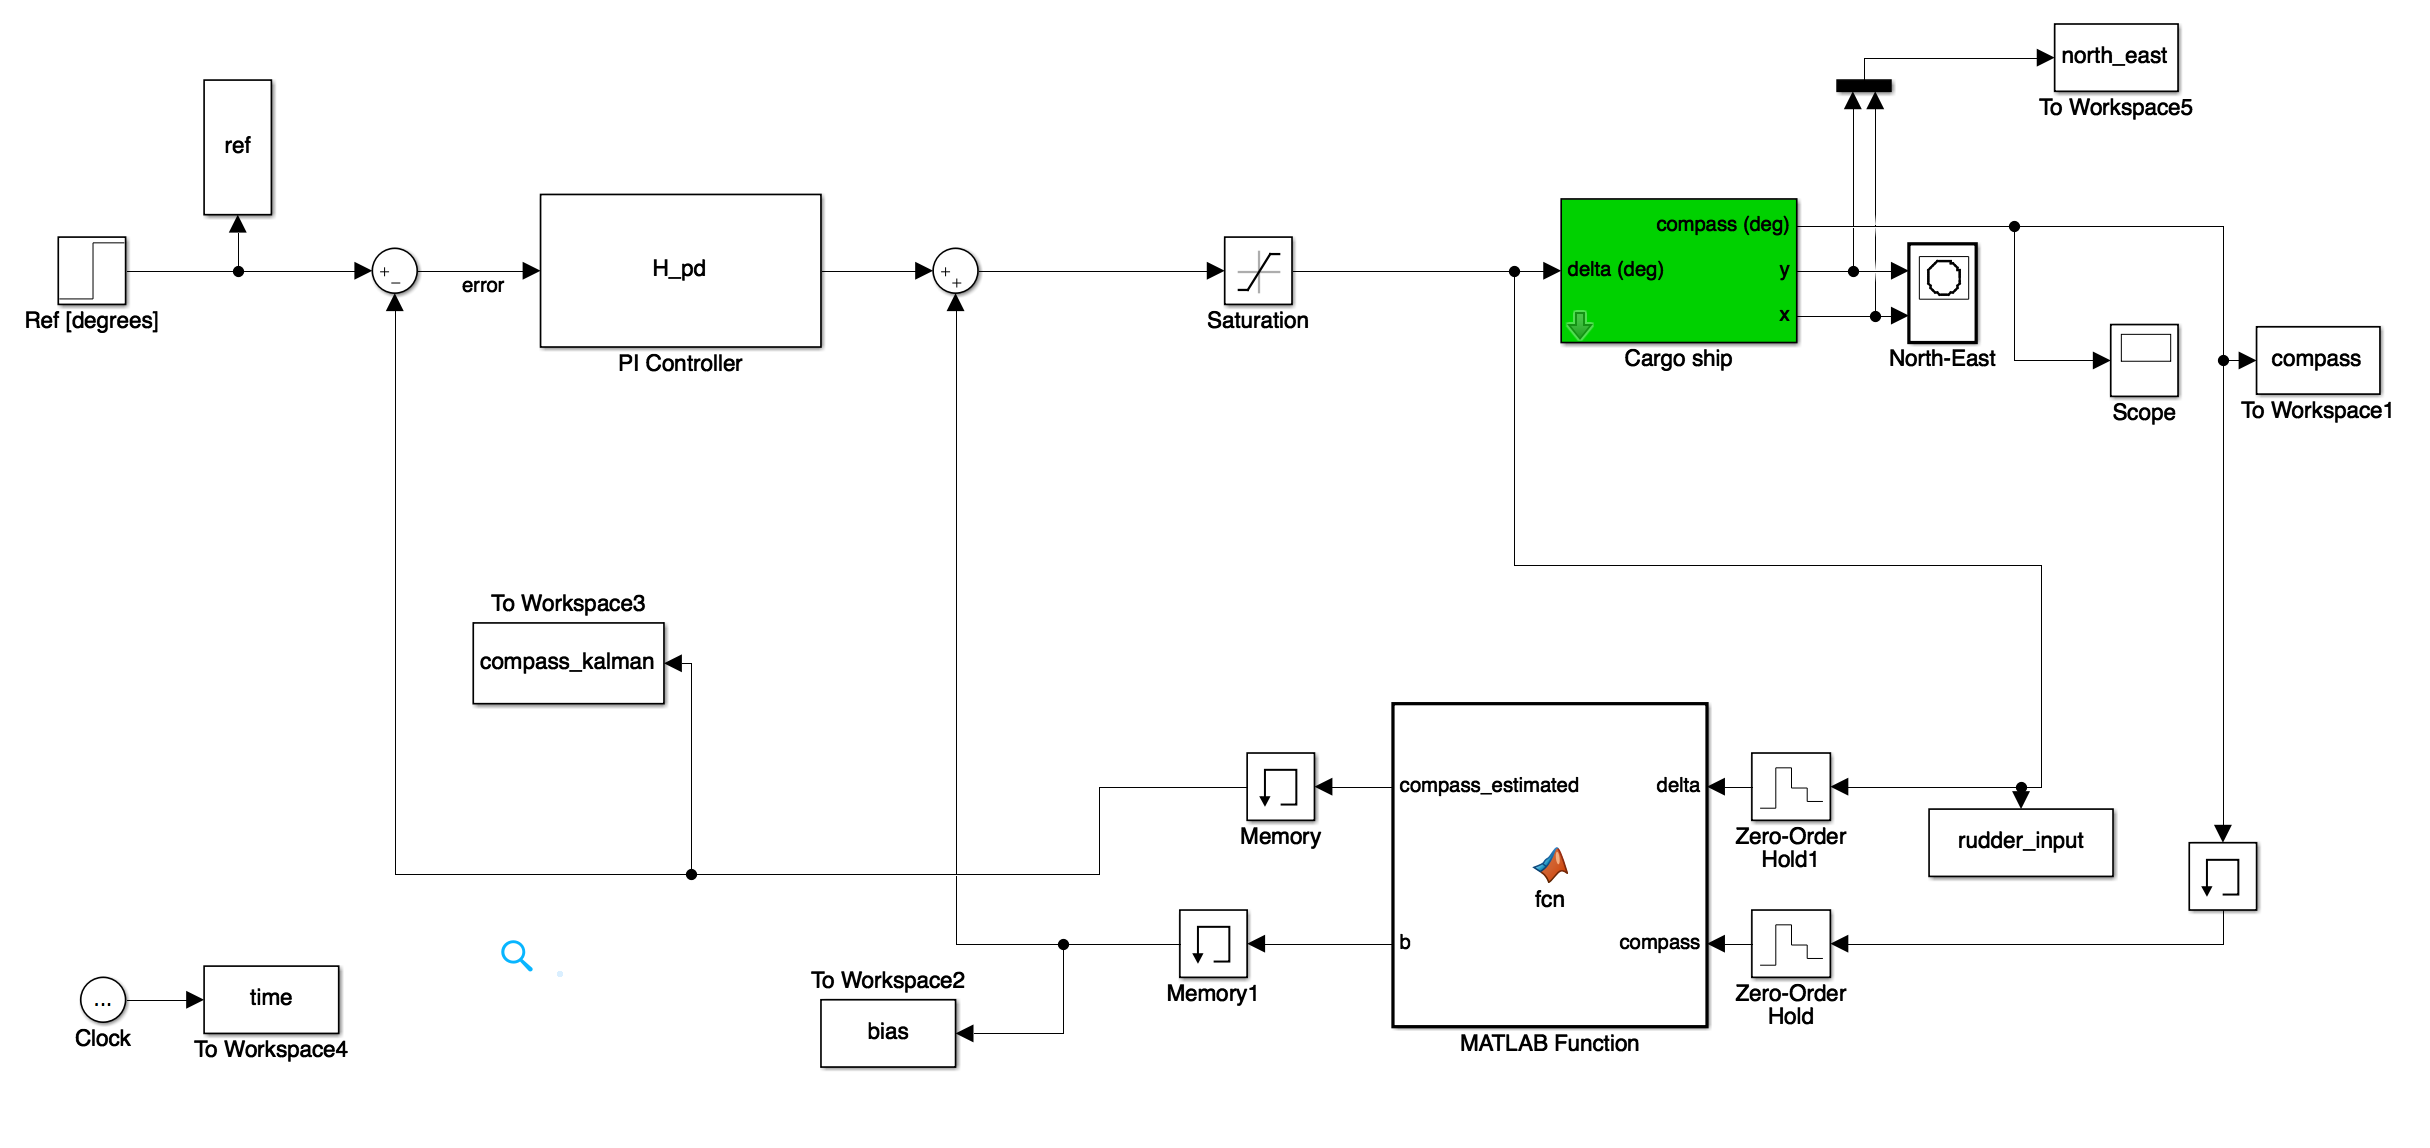
\includegraphics[scale=0.3]{simulink/sim5e}}

\end{figure}
